\documentclass[11pt,a4paper,oneside]{report}
\usepackage[a4paper,margin=27mm,headheight=15pt]{geometry}
\usepackage[T1]{fontenc}
\usepackage{tgpagella}
\usepackage{microtype}
\usepackage{graphicx}
\usepackage{booktabs}
\usepackage{array}
\usepackage[table]{xcolor}
\usepackage{caption}
\usepackage{fancyhdr}
\usepackage[hidelinks]{hyperref}
\definecolor{accent}{HTML}{214F70}
\definecolor{soft}{HTML}{E9F1F5}
\definecolor{headerblue}{HTML}{214F70}
\definecolor{rowgray}{HTML}{E9F1F5}
\hypersetup{pdftitle={Spam Email Classifier: A Personal Project Report},pdfauthor={Mohamed Aassou},colorlinks=true,linkcolor=accent,urlcolor=accent,citecolor=accent}
\captionsetup{font=small,labelfont=bf}
\setlength{\parindent}{0pt}
\setlength{\parskip}{0.55em}
\pagestyle{fancy}
\fancyhf{}
\fancyhead[L]{\small Personal project report}
\fancyhead[R]{\small Mohamed Aassou}
\fancyfoot[L]{\small\color{accent}Spam Email Classifier}
\fancyfoot[R]{\thepage}
\renewcommand{\headrulewidth}{0.4pt}
\renewcommand{\footrulewidth}{0.4pt}
\fancypagestyle{plain}{%
  \fancyhf{}
  \fancyfoot[L]{\small\color{accent}Spam Email Classifier}
  \fancyfoot[R]{\thepage}
  \renewcommand{\headrulewidth}{0pt}
  \renewcommand{\footrulewidth}{0.4pt}}
\fancypagestyle{cover}{%
  \fancyhf{}
  \fancyfoot[C]{\small\color{accent}Spam Email Classifier}
  \renewcommand{\headrulewidth}{0pt}
  \renewcommand{\footrulewidth}{0pt}}
\newcommand{\reportfigure}[4]{%
  \begin{figure}[p]\centering
  \includegraphics[width=#3\textwidth,height=0.72\textheight,keepaspectratio]{assets/#1}
  \caption{#2}\label{#4}
  \end{figure}}
\begin{document}
\hypersetup{pageanchor=false}
\begin{titlepage}
\thispagestyle{cover}
\centering
\vspace*{2.6cm}
{\color{accent}\rule{0.65\textwidth}{1.3pt}}\par\vspace{0.8cm}
{\Huge\bfseries Spam Email Classifier\par}
\vspace{0.4cm}
{\Large From email data to a working classifier\par}
\vspace{0.9cm}
{\color{accent}\rule{0.65\textwidth}{1.3pt}}\par
\vfill
{\large A personal project report\par}
\vspace{1cm}
\renewcommand{\arraystretch}{1.35}
\begin{tabular}{>{\bfseries}p{35mm}p{72mm}}
\rowcolor{headerblue}\multicolumn{2}{c}{\color{white}\bfseries Project details}\\
\rowcolor{rowgray}Author & Mohamed Aassou\\
\rowcolor{white}Project & Spam Email Classifier\\
\rowcolor{rowgray}Source & \href{https://github.com/mohammedaassou/Spam-Email-Classifier}{GitHub repository}\\
\end{tabular}
\vspace*{1.8cm}
\end{titlepage}
\hypersetup{pageanchor=true}
\pagenumbering{roman}
\chapter*{Abstract}
\addcontentsline{toc}{chapter}{Abstract}
This report describes my personal Spam Email Classifier project. I prepared a public collection of emails, compared several ways to distinguish spam from legitimate messages, and built a small web page that shows a prediction. The examined dataset contains 2,998 messages before repeated emails are removed. On the reserved final test set, the chosen model classified 586 of 590 messages correctly. The report explains what these results show, where the current application stops, and why performance on this older collection may not reflect present-day email.
\tableofcontents
\listoffigures
\clearpage\pagenumbering{arabic}
\chapter{Introduction and project scope}
\section{Why this project matters}
Spam wastes attention and can contain deceptive offers or requests. A filter can help, but its mistakes matter: a legitimate message might be marked as spam, while an unwanted one might still reach the inbox. I built this project to learn how an email classifier is prepared, evaluated and made available through a simple web page. A person enters a subject and message body and receives a spam or legitimate result. The project does not connect to an inbox or move messages automatically.

The work uses two parts of the public SpamAssassin email collection: one containing ordinary messages and one containing spam\cite{corpus}. An early project note names 97\% accuracy as a goal. The results in this report come from the saved evaluation figures and are presented separately from that goal. The source is available in the \href{https://github.com/mohammedaassou/Spam-Email-Classifier}{project's GitHub repository}.

\section{Project goals}
The main goal is to make a useful prediction from an email's subject and body. I also wanted a fair comparison between a simple starting point and several learning models. Table~\ref{tab:req} shows what the current project does and what is still planned.

\begin{center}\small
\captionof{table}{Project goals and current state}\label{tab:req}
\renewcommand{\arraystretch}{1.08}
\begin{tabular}{>{\raggedright\arraybackslash}p{31mm}>{\raggedright\arraybackslash}p{83mm}>{\raggedright\arraybackslash}p{24mm}}\toprule
\rowcolor{headerblue}\textcolor{white}{\bfseries Goal} & \textcolor{white}{\bfseries What it means} & \textcolor{white}{\bfseries State}\\\midrule
\rowcolor{rowgray}Enter an email & Supply a subject and body; reject empty entries. & Available\\
\rowcolor{white}Classify it & Return spam or legitimate mail. & Available\\
\rowcolor{rowgray}See the answer & Show the result on the web page. & Available\\
\rowcolor{white}Show confidence & Display the estimated chance of spam. & Planned\\
\rowcolor{rowgray}Compare fairly & Choose a model before using the reserved final test set. & Available\\
\rowcolor{white}Measure speed & Record how long predictions take. & Planned\\\bottomrule
\end{tabular}
\end{center}

\clearpage
\section{Technologies used}
The project uses a small set of tools for preparing email data, comparing models, showing results and serving the web page. Their official logos are shown in Table~\ref{tab:technology}.

\begin{center}\small
\captionof{table}{Main technologies used in the project}\label{tab:technology}
\renewcommand{\arraystretch}{1.35}
\begin{tabular}{>{\centering\arraybackslash}m{37mm}>{\raggedright\arraybackslash}m{99mm}}\toprule
\rowcolor{headerblue}\textcolor{white}{\bfseries Official logo} & \textcolor{white}{\bfseries Role in the project}\\\midrule
\rowcolor{rowgray}\colorbox{white}{
\includegraphics[width=32mm,height=15mm,keepaspectratio]{assets/logo_python.png}} & \textbf{\href{https://www.python.org/}{Python}} is the language used to build the classifier and the web application.\\
\rowcolor{white}\colorbox{white}{
\includegraphics[width=32mm,height=15mm,keepaspectratio]{assets/logo_pandas.png}} & \textbf{\href{https://pandas.pydata.org/}{pandas}} helps read, inspect and prepare the email collection.\\
\rowcolor{rowgray}\colorbox{white}{
\includegraphics[width=32mm,height=15mm,keepaspectratio]{assets/logo_scikit_learn.png}} & \textbf{\href{https://scikit-learn.org/}{scikit-learn}} provides the text features, learning models and evaluation tools.\\
\rowcolor{white}\colorbox{white}{
\includegraphics[width=32mm,height=15mm,keepaspectratio]{assets/logo_fastapi.png}} & \textbf{\href{https://fastapi.tiangolo.com/}{FastAPI}} connects the web page to the saved classifier.\\
\rowcolor{rowgray}\colorbox{white}{
\includegraphics[width=32mm,height=15mm,keepaspectratio]{assets/logo_matplotlib.png}} & \textbf{\href{https://matplotlib.org/}{Matplotlib}} helps create charts for data exploration and model evaluation.\\\bottomrule
\end{tabular}
\end{center}

The project also uses NLTK to prepare words, Jinja2 to display the web page and Uvicorn to run the web service.

\chapter{The email data}
\section{Source and balance}
The project draws on two publicly available SpamAssassin collections\cite{corpus}. It extracts each email's subject and plain-text body and stores them for analysis. The dataset examined for this report contains 2,998 emails: 2,500 legitimate messages and 498 spam messages. Figure~\ref{fig:class} shows this imbalance. A classifier that always says ``legitimate'' would be right often, but it would fail to catch every spam email. That is why the later comparison looks beyond overall accuracy.

The examined data also contains 49 repeated subject-and-body pairs, two empty subjects and 212 empty bodies. No identical pair carries conflicting labels. These numbers describe the saved dataset used for inspection; a fresh download or different parsing method could produce different counts.

\reportfigure{class_distribution.png}{Messages in the examined dataset before repeated emails are removed. Legitimate mail makes up 83.4\% of the total.}{0.86}{fig:class}

\section{Preparing the messages}
Missing subjects or bodies are treated as empty text. The project makes labels consistent, checks for contradictory labels on identical emails, and removes repeated subject-and-body pairs. This leaves 2,949 distinct pairs: 2,472 legitimate messages and 477 spam messages. Removing exact repeats before dividing the data prevents the same email from appearing in both learning and evaluation groups.

For each remaining email, the subject and body are joined. The text is changed to lowercase, punctuation and numbers are removed, common English words are dropped, and related word forms are reduced to a common stem. A separate word-weighting step then gives more influence to words that help distinguish messages; this method is known as TF-IDF\cite{tfidf}. The word weights are learned only from the messages used to train a model\cite{pipeline}. Similar but non-identical emails can still appear in different groups.

\chapter{How the models were compared}
\section{Keeping evaluation separate}
The prepared emails are divided into three groups while keeping a similar share of spam in each. About 64\% are used to fit the candidate models, 16\% to compare them, and 20\% are held back for a final test. The comparison group contains 472 emails (396 legitimate, 76 spam); the final test group contains 590 (495 legitimate, 95 spam). Figure~\ref{fig:trainflow} gives a visual overview. It simplifies the process, so the three group sizes and the final retraining step are explained here.

\reportfigure{training_flow.png}{Learning process: compare models, train the chosen one again, then run the final test.}{0.95}{fig:trainflow}

The starting point is a model that always chooses the most common group. Three other approaches use weighted words: Naive Bayes, Logistic Regression and a linear Support Vector Machine (SVM). Each one learns from the first group, then makes predictions for the separate comparison group. The word weights are learned alongside each model, so the comparison and final test messages do not influence that learning\cite{pipeline}.

\section{Choosing the final model}
The comparison uses three measures focused on spam. \emph{Precision} asks how often a spam warning is right. \emph{Recall} asks how much real spam is caught. \emph{F1} combines both into one score. The project uses Logistic Regression as its final model. This choice is set in the project rather than selected automatically from the comparison results. The model is then trained again using the combined 80\% learning portion and saved for later predictions. Only after that does the project evaluate it on the untouched final test group.

\chapter{What the evaluation showed}
\section{Comparing the models}
Figure~\ref{fig:compare} compares the models on the same validation group. The simple model that always chooses the majority class catches no spam. Naive Bayes catches eight of 76 spam emails but misses the other 68. Logistic Regression and SVM perform equally in the saved results: both catch 70 spam emails, miss six, and wrongly flag one legitimate email. Their displayed precision, recall and F1 scores are therefore tied. The project proceeds with Logistic Regression, which can also estimate a chance of spam, although the current web page does not show that estimate.

\reportfigure{model_comparison_readable.png}{Comparison results for the models before the final test. Logistic Regression and SVM have the same scores in this figure.}{0.95}{fig:compare}

Figures~\ref{fig:dummy}--\ref{fig:svm} show the mistakes behind the summary chart. In each matrix, the rows are the real labels and the columns are the predicted labels. These figures belong to the model comparison stage; they are separate from the final test.

\reportfigure{validation_majority_readable.png}{Validation results for the majority-choice starting point: it misses all 76 spam emails.}{0.75}{fig:dummy}
\reportfigure{validation_nb.png}{Naive Bayes comparison: eight spam emails caught and 68 missed.}{0.75}{fig:nb}
\reportfigure{validation_logreg.png}{Logistic Regression comparison: one false alarm and six missed spam emails.}{0.75}{fig:logreg}
\reportfigure{validation_svm.png}{Validation results for SVM: the same recorded mistake counts as Logistic Regression.}{0.75}{fig:svm}

\section{Testing the chosen model}
On the reserved test group, the chosen model classifies 493 legitimate emails and 93 spam emails correctly. It wrongly flags two legitimate emails and misses two spam emails, as Figure~\ref{fig:test} shows. That is 586 correct answers out of 590, or about 99.32\% accuracy. For spam specifically, both precision and recall are about 97.89\%; F1 is also about 97.89\%. These results apply to this test group and do not establish how well the model would handle today's incoming mail.

Figure~\ref{fig:roc} shows how the model separates the two groups across different decision levels. Its displayed summary score rounds to 1.00. The figure does not provide the more precise value, so none is claimed here.

\reportfigure{test_matrix.png}{Final test results: 493 legitimate and 93 spam emails classified correctly, with four mistakes in total.}{0.78}{fig:test}
\reportfigure{roc_curve.png}{Final test curve showing how well the chosen model separates spam from legitimate mail at different decision levels.}{0.72}{fig:roc}

\chapter{Using the classifier}
\section{From email to result}
The web page asks for a subject and message body. It checks that neither field is empty, then sends the text to a small FastAPI service. The service prepares the text in the same general way as the training data, asks the saved model for a prediction, and returns ``spam'' or ``legitimate.'' The page then shows the result with a short explanation. A chance of spam can be calculated inside the application, but it is not currently included in what the user sees.

Figure~\ref{fig:predicta} illustrates that path. Its final ``Spam probability'' label describes a planned addition, not the current screen. Figure~\ref{fig:screen} shows the page before an email has been checked. It documents the interface rather than a completed prediction.

\reportfigure{prediction_flow_a.png}{The email prediction journey. Showing a spam probability is still planned.}{0.95}{fig:predicta}
\reportfigure{screen_home.png}{Home page with spaces for the email subject and body and a panel for the result.}{0.70}{fig:screen}

\section{Current limits of the application}
The application reads the saved model again for each prediction. That makes the design simple, but it may add delay; no timing study has been recorded. The project has a local web interface, with no evidence here of a hosted service. A few example emails are included for demonstration, but they are not a substitute for the separate evaluation set.

\chapter{Limits and next steps}
The final test contains two legitimate emails marked as spam and two spam emails allowed through. The saved chart shows how many mistakes occurred, but the project does not yet examine the actual messages behind them. Reviewing those emails would show whether particular words, writing styles or message lengths caused trouble. It would also help decide whether the classifier should be more cautious about blocking legitimate mail or more aggressive about catching spam.

The data comes from an older public collection. Its legitimate messages come from the ``easy ham'' group, which the corpus notes is relatively easy to distinguish from spam\cite{corpus}. The strong test result may therefore be optimistic for modern or unfamiliar email. The project has no separate collection from another time or source for a broader check. Repeated identical emails were removed before evaluation, but very similar messages may remain in different groups.

There is also a small difference between learning and prediction: the prepared learning messages include words identifying the subject and body, while the text sent for a new prediction does not. The project should prepare both in exactly the same way. Future work could also show the estimated chance of spam, examine different decision levels, study mistakes one message at a time, record prediction speed, and test on newer email. These are next steps, not features claimed as complete.

\chapter{Conclusion}
This personal project follows the full path from collecting email data to showing a classification on a web page. The saved comparison shows that the learned models improve greatly on always choosing the most common group. Logistic Regression and SVM tie in the displayed comparison, and the chosen Logistic Regression model makes four mistakes among 590 messages in the reserved final test. The result is promising for this collection, while the age and limited variety of the data leave an important question: how well would it work on new kinds of email? A broader test and a closer look at mistakes are the most useful next steps.

\appendix
\chapter{Supplementary visual material}
Figure~\ref{fig:predictb} shows another version of the prediction journey. Its ``Spam probability'' label refers to a planned feature. The current page shows only the classification.
\begin{figure}[htbp]\centering
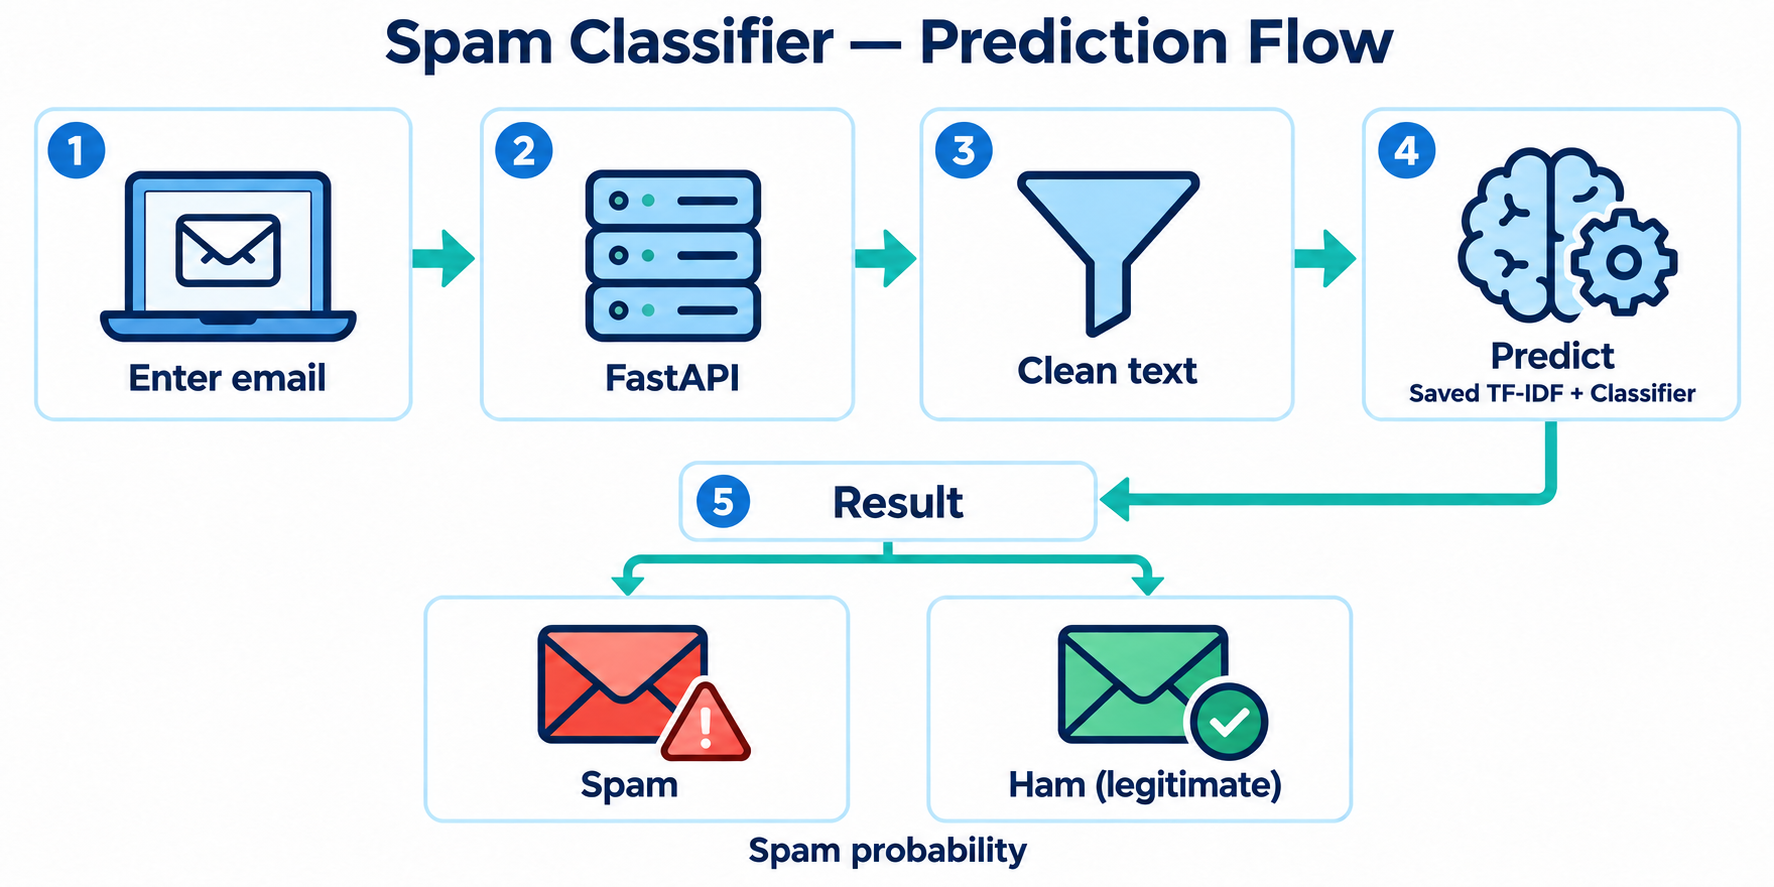
\includegraphics[width=0.95\textwidth,height=0.38\textheight,keepaspectratio]{assets/prediction_flow_b.png}
\caption{Another view of the prediction journey. The probability display is planned.}\label{fig:predictb}
\end{figure}


\begin{thebibliography}{9}
\addcontentsline{toc}{chapter}{References}
\bibitem{corpus} Apache SpamAssassin, ``\href{https://spamassassin.apache.org/old/publiccorpus/readme.html}{Public Corpus README}'' and \href{https://spamassassin.apache.org/old/publiccorpus/}{archive index}. Accessed 28 October 2026.
\bibitem{pipeline} scikit-learn developers, ``\href{https://scikit-learn.org/stable/getting_started.html}{Getting Started: Estimators and pipelines}.'' Accessed 28 October 2026.
\bibitem{tfidf} scikit-learn developers, ``\href{https://scikit-learn.org/stable/modules/generated/sklearn.feature_extraction.text.TfidfVectorizer.html}{TfidfVectorizer documentation}.'' Accessed 28 October 2026.
\end{thebibliography}

\end{document}
